\documentclass[runningheads]{llncs}

%PACKAGES
\usepackage[utf8]{inputenc}
\usepackage{listings, xcolor}
\usepackage{graphicx} 
\usepackage{lipsum}
\setcounter{secnumdepth}{5}
\begin{document}
\title{Comparing Go, FreeST and Rust}
\author{Jorge Martins\inst{1} \and
Diogo Lopes\inst{1}
}
\definecolor{darkblue}{rgb}{0.0, 0.0, 0.55}
\lstset{language=Java,
numbers=none,
keywordstyle = \color{blue},
commentstyle = \color{darkblue},
breaklines = true,
showstringspaces = false,
tabsize = 4,
basicstyle=\small,
} 
\institute{Departamento de Informática da Faculdade de Ciências da Universidade de Lisboa
\email{\{fc51033,fc51058\}@alunos.fc.ul.pt}}
\nocite{*}
\maketitle
\thispagestyle{empty}
\begin{abstract}
\lipsum[1]
\end{abstract}
\section{Introduction}
\lipsum
\newpage
\section{Background}
\subsection{The Plane Ticket Algorithm}
\begin{figure}
\centering
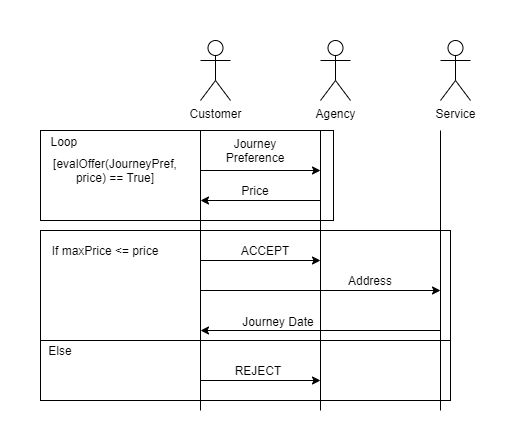
\includegraphics[scale=0.4]{Algorithm.png}
\caption{Plane Ticket Algorithm System Sequence Diagram}
\end{figure}
\begin{lstlisting}[caption={Customer Algorithm},captionpos=b]
class Customer {
	Address addr;
	double price, maxPrice;
	bool loop := true;
	String journeyPref;
	new Agency.sell {
		sendWhile (loop) {
			send( journeyPref );
			price := receive;
			loop := evalOffer(journeyPref,price);
			// implementation of evalOffer omitted
		};
		sendCase( evalPrice(price,maxPrice) ) {
			ACCEPT > send( addr ); Date date := receive;
			REJECT > null; /* customer rejects price
					,end of protocol */ 
		}
	} /* End method invocation */
}
\end{lstlisting}
\newpage
\begin{lstlisting}[caption={Agency Algorithm},captionpos=b]
class Agency {
	String journeyPref;
	void acceptOrder sell {
		receiveWhile {
			journeyPref := receive;
			double price := getPrice( journeyPref );
			// implementation of getPrice omitted
			send( price );
		}
		receiveCase (x) { // buyer accepts price
			ACCEPT < new Service . orderDelivery { } ,
			REJECT < null;// receiveCase : buyer rejects 
        }
	} /* End method sell */
}
\end{lstlisting}
\begin{lstlisting}[caption={Service Algorithm},captionpos=b]
class Service {
	void receiveOrderSession orderDelivery() {
		Address custAddress := receive;
		Date date := new Date();
		send( date );
	}
}
\end{lstlisting}
\subsection{Programming Languages}
\subsubsection{Rust}\hfill\\\\
\subsubsection{Go}\hfill\\\\
\subsubsection{FreeST}\hfill\\\\
\lipsum[1]
\section{Implementation Details}
\lipsum[1]
\subsection{Go}
\lipsum[1]
\subsection{Rust}
\lipsum[1]
\subsection{FreeST}
\lipsum[1]
\subsection{Evaluation}
\lipsum[1]
\section{Conclusions}
\lipsum
\section*{Acknowledgements}
\lipsum[1]
\bibliographystyle{unsrt}
\bibliography{bibliography}
\end{document}